% ScoutAI — Technical Report
% Build:  pdflatex -interaction=nonstopmode technical-report.tex   (run twice)
\documentclass[11pt,a4paper]{article}

% --- Fonts and typography -------------------------------------------------
\usepackage[T1]{fontenc}
\usepackage[utf8]{inputenc}
\usepackage{newtxtext,newtxmath}
\usepackage[varqu,varl,scaled=0.95]{inconsolata}
\usepackage{microtype}

% --- Page ------------------------------------------------------------------
\usepackage[a4paper,margin=1.05in,top=1.1in,bottom=1.15in]{geometry}
\usepackage{fancyhdr}
\usepackage{titlesec}
\usepackage{enumitem}
\setlist{itemsep=1pt,topsep=3pt,parsep=0pt}

% --- Tables and figures ----------------------------------------------------
\usepackage{booktabs}
\usepackage{array}
\usepackage{tabularx}
\usepackage{makecell}
\usepackage{float}
\usepackage[section]{placeins}
\usepackage[font=small,labelfont=bf,width=0.94\textwidth]{caption}

% --- Graphics --------------------------------------------------------------
\usepackage{adjustbox}
\usepackage{xcolor}
\usepackage{tikz}
\usetikzlibrary{positioning,arrows.meta,calc,fit,backgrounds,shapes.geometric,
                decorations.pathreplacing}

% --- Links -----------------------------------------------------------------
\definecolor{linknavy}{HTML}{1F4E79}
\usepackage[colorlinks=true,linkcolor=linknavy,urlcolor=linknavy,
            citecolor=linknavy,pdftitle={ScoutAI: Architecture and Engineering
            Decisions},pdfauthor={Sai Nikhil Kunapareddy}]{hyperref}

% --- Palette ---------------------------------------------------------------
\definecolor{cCore}{HTML}{1F4E79}   % the agent core
\definecolor{cTool}{HTML}{A4601F}   % tools and the outside world
\definecolor{cState}{HTML}{2F6B4F}  % anything persisted
\definecolor{cInfra}{HTML}{545A66}  % process and platform
\definecolor{cWarn}{HTML}{9B2C2C}   % failure paths
\definecolor{cEdge}{HTML}{3D3D3D}

% --- One visual language for every figure ---------------------------------
\tikzset{
  >={Stealth[round,length=2.1mm,width=1.7mm]},
  box/.style   ={draw=cEdge!65, line width=0.5pt, rounded corners=2pt,
                 fill=white, align=center, inner sep=3.2pt,
                 minimum height=7.6mm, font=\small},
  core/.style  ={box, draw=cCore!75, fill=cCore!7,  text=cEdge},
  tool/.style  ={box, draw=cTool!80, fill=cTool!8,  text=cEdge},
  state/.style ={box, draw=cState!80, fill=cState!8, text=cEdge},
  infra/.style ={box, draw=cInfra!75, fill=cInfra!7, text=cEdge},
  ext/.style   ={box, draw=cInfra!55, fill=white, densely dashed, text=cEdge},
  warn/.style  ={box, draw=cWarn!75, fill=cWarn!6,  text=cEdge},
  term/.style  ={draw=cEdge!65, line width=0.5pt, rounded corners=8pt,
                 fill=cEdge!5, align=center, inner sep=3pt,
                 minimum height=6.4mm, font=\small\scshape},
  dec/.style   ={draw=cCore!75, line width=0.5pt, fill=cCore!5, align=center,
                 inner sep=3pt, minimum height=7mm, font=\small\itshape,
                 rounded corners=1pt},
  flow/.style  ={->, draw=cEdge!85, line width=0.55pt},
  back/.style  ={->, draw=cEdge!70, line width=0.55pt, densely dashed},
  fail/.style  ={->, draw=cWarn!85, line width=0.6pt},
  lbl/.style   ={font=\scriptsize, text=cEdge!85, inner sep=1.6pt,
                 fill=white, rounded corners=1pt},
  faillbl/.style={font=\scriptsize, text=cWarn, inner sep=1.6pt, fill=white},
  grp/.style   ={draw=cInfra!40, densely dashed, rounded corners=3pt,
                 inner sep=3.6mm},
  grplbl/.style={font=\scriptsize, text=cInfra, inner sep=1.5pt,
                 fill=white},
  life/.style  ={draw=cEdge!40, densely dotted, line width=0.5pt},
}

% --- Section styling -------------------------------------------------------
\titleformat{\section}{\normalfont\large\bfseries}{\thesection}{0.7em}{}
\titleformat{\subsection}{\normalfont\normalsize\bfseries}{\thesubsection}{0.6em}{}
\titlespacing*{\section}{0pt}{14pt plus 3pt minus 2pt}{6pt}
\titlespacing*{\subsection}{0pt}{10pt plus 2pt minus 2pt}{4pt}

\pagestyle{fancy}
\fancyhf{}
\fancyhead[L]{\small\scshape ScoutAI --- Architecture and Engineering Decisions}
\fancyhead[R]{\small\thepage}
\renewcommand{\headrulewidth}{0.3pt}

\newcolumntype{L}[1]{>{\raggedright\arraybackslash}p{#1}}
\newcommand{\tablefont}{\footnotesize}

\title{\vspace{-1.2cm}\textbf{ScoutAI: A Multi-Agent Job-Search Platform\\on LangGraph}\\[2mm]
  \large Architecture, Engineering Decisions, and Their Costs}
\author{Sai Nikhil Kunapareddy}
\date{\today}

\begin{document}
\maketitle
\thispagestyle{fancy}

\begin{abstract}
\noindent
Scout is a multi-agent platform that runs job-search assistants as Slack direct-message
bots. An agent is a declarative specification --- a system prompt and a set of tools ---
compiled onto a single shared LangGraph model/tool loop and served to many users from one
process, on any of three interchangeable model backends. The platform covers 29 companies
through 16 source modules that share no upstream API, tailors every search to the user's
résumé through a two-stage graph whose cache \emph{is} its checkpointed state, and scopes
one agent entirely to the companies where the user has a referral.

This report describes the architecture and, more importantly, the decisions behind it and
what each one cost: why conversation history lives in a checkpointer thread rather than in
application state; why an unreachable job board must never be reported as an empty one;
why company-to-board routing is a lookup table rather than a prompt; why a model retry
belongs inside the graph node and not around the turn; and why a turn that runs out of tool
hops must repair its own thread before apologising. It closes with the system's limits and
the specific constraint each next step would remove.
\end{abstract}

\vspace{2mm}
{\small\tableofcontents}
\vspace{4mm}

% ==========================================================================
\section{Problem and scope}
% ==========================================================================

An AI/ML job search looks like a generation problem and is almost entirely a data
integration problem. The roles worth seeing are spread across a few dozen company careers
boards that share no API and no common format: some publish a JSON endpoint that their own
single-page app consumes, some publish RSS and nothing else, and some publish only
server-rendered HTML. None of them rank results against a particular résumé, and none of
them know that the person searching has a former colleague at Stripe --- which is, in
practice, the single strongest signal about whether an application goes anywhere.

Scout was built against six requirements:

\begin{enumerate}[label=\textbf{R\arabic*.},leftmargin=2.4em]
  \item \textbf{Tailored.} Every search is shaped by the user's own résumé, without the
    user restating it.
  \item \textbf{Referral-aware.} A role at a company where the user knows someone outranks
    a marginally better-matched role where they know nobody.
  \item \textbf{Scope-complete.} One agent answers ``what is open where I could ask for a
    referral'' and, when it cannot check something, says so rather than returning a
    quietly short list.
  \item \textbf{Unprompted.} A digest arrives every morning without anyone typing anything.
  \item \textbf{Cheap.} It runs on an AWS free-tier \texttt{t4g.micro} (2 vCPU, 916\,MB, no
    swap).
  \item \textbf{Portable across models.} A hosted Claude outage, a rate limit, or a cost
    spike must not be a dead bot; a local model must be one message away.
\end{enumerate}

Explicit non-goals: applying on the user's behalf, multi-tenant SaaS, and a web front end.

Slack DMs were chosen as the entire interface because a DM is three things at once --- an
input channel, a notification channel, and an identity --- so R4 costs nothing extra and no
front end has to be written, authenticated, or hosted. The cost of that choice is a 3{,}500
character practical message limit and no rich interaction beyond text, which is why replies
are split on line boundaries and never on characters (a hard split would break a job link).

% ==========================================================================
\section{The system at a glance}
% ==========================================================================

Figure~\ref{fig:context} is the whole system on one page. Table~\ref{tab:agents} is the
agent catalogue and Table~\ref{tab:backends} the model backends. In numbers: 6{,}265 lines
of Python in the package, 5{,}593 lines of tests, 389 tests, 100\,\% statement \emph{and}
branch coverage enforced in CI across Python 3.10--3.13, running as six systemd units on
one machine.

\begin{figure}[!ht]
\centering
\begin{adjustbox}{max width=\textwidth}
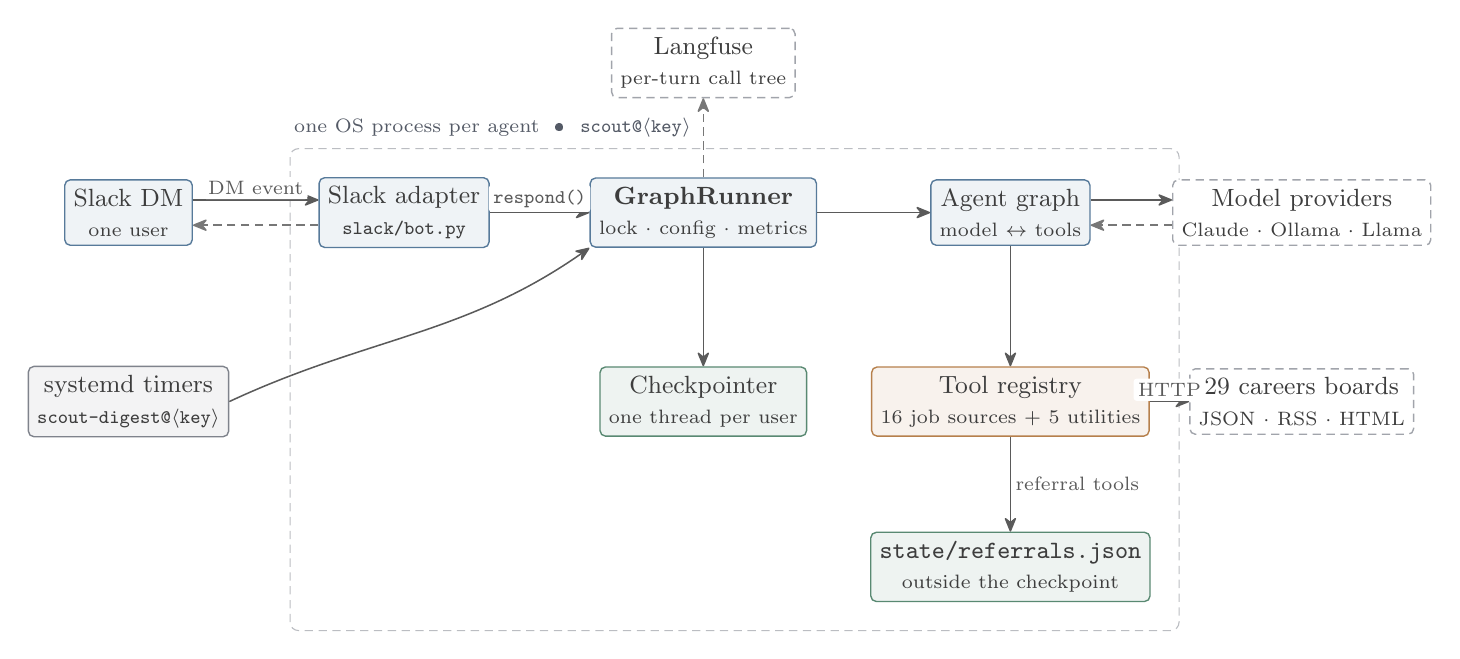
\begin{tikzpicture}[x=1cm,y=1cm]
  \node[core]  (user)   at (0,0)      {Slack DM\\\scriptsize one user};
  \node[core]  (bot)    at (3.5,0)    {Slack adapter\\\scriptsize\texttt{slack/bot.py}};
  \node[core]  (runner) at (7.3,0)    {\textbf{GraphRunner}\\\scriptsize lock $\cdot$ config $\cdot$ metrics};
  \node[core]  (graph)  at (11.2,0)   {Agent graph\\\scriptsize model $\leftrightarrow$ tools};
  \node[ext]   (prov)   at (14.9,0)   {Model providers\\\scriptsize Claude $\cdot$ Ollama $\cdot$ Llama};
  \node[ext]   (lf)     at (7.3,1.9)  {Langfuse\\\scriptsize per-turn call tree};
  \node[state] (ckpt)   at (7.3,-2.4) {Checkpointer\\\scriptsize one thread per user};
  \node[tool]  (tools)  at (11.2,-2.4){Tool registry\\\scriptsize 16 job sources $+$ 5 utilities};
  \node[ext]   (boards) at (14.9,-2.4){29 careers boards\\\scriptsize JSON $\cdot$ RSS $\cdot$ HTML};
  \node[state] (refs)   at (11.2,-4.5){\texttt{state/referrals.json}\\\scriptsize outside the checkpoint};
  \node[infra] (timer)  at (0,-2.4)   {systemd timers\\\scriptsize\texttt{scout-digest@$\langle$key$\rangle$}};

  \draw[flow] ([yshift=1.6mm]user.east)  -- node[lbl,above]{\scriptsize DM event} ([yshift=1.6mm]bot.west);
  \draw[back] ([yshift=-1.6mm]bot.west)  -- ([yshift=-1.6mm]user.east);
  \draw[flow] (bot) -- node[lbl,above]{\scriptsize\texttt{respond()}} (runner);
  \draw[flow] (runner) -- (graph);
  \draw[flow] ([yshift=1.6mm]graph.east) -- ([yshift=1.6mm]prov.west);
  \draw[back] ([yshift=-1.6mm]prov.west) -- ([yshift=-1.6mm]graph.east);
  \draw[flow] (graph) -- (tools);
  \draw[flow] (tools) -- node[lbl,above]{\scriptsize HTTP} (boards);
  \draw[flow] (runner) -- (ckpt);
  \draw[flow] (tools) -- node[lbl,right]{\scriptsize referral tools} (refs);
  \draw[back] (runner) -- (lf);
  \draw[flow] (timer.east) to[out=25,in=215] (runner.south west);

  \begin{scope}[on background layer]
    \node[grp, fit=(bot)(runner)(graph)(tools)(ckpt)(refs)] (proc) {};
  \end{scope}
  \node[grplbl, anchor=south west] at ([yshift=0.8mm]proc.north west)
    {one OS process per agent \ \textbullet\ \ \texttt{scout@$\langle$key$\rangle$}};
\end{tikzpicture}
\end{adjustbox}
\caption{System context. Everything inside the dashed boundary is one Python process holding
one Slack app's token; a second agent is a second process, not a second code path. Two things
cross the boundary in both directions --- model calls and Slack messages --- and two only
leave it: job-board HTTP and observability.}
\label{fig:context}
\end{figure}

\begin{table}[!ht]
\centering\tablefont
\caption{The four registered agents. Adding one is a single file plus one registry line;
nothing about the graph changes.}
\label{tab:agents}
\begin{tabularx}{\textwidth}{L{2.1cm} L{3.5cm} X c c}
\toprule
\textbf{Key} & \textbf{Name} & \textbf{Tools} & \makecell{\textbf{Résumé-}\\\textbf{tailored}}
& \makecell{\textbf{In daily}\\\textbf{digest}} \\
\midrule
\texttt{bigtech} & BigTech Agent & clock, location, \texttt{referrals\_\allowbreak{}read}, 14 job-source
  modules covering 27 companies & yes & yes \\
\texttt{edu} & Edu Agent & clock, location, \texttt{referrals\_\allowbreak{}read}, Northeastern, Boston
  University & yes & yes \\
\texttt{referral} & Referral Window & clock, \texttt{referrals} (read \emph{and} write),
  \texttt{search\_\allowbreak{}referral\_\allowbreak{}jobs} & no & yes \\
\texttt{resume} & Resume Parser & \texttt{get\_\allowbreak{}resume\_\allowbreak{}profile} & n/a & no \\
\bottomrule
\end{tabularx}
\end{table}

Two things in Table~\ref{tab:agents} are load-bearing rather than incidental. First, the
job agents get \texttt{referrals\_\allowbreak{}read} and the Referral Window gets \texttt{referrals}:
only one agent may write the list, because an agent with \texttt{add\_\allowbreak{}referral} within reach
will eventually record something mid-search that the user never asked for. Second,
``résumé-tailored'' and ``in digest'' are separate flags even though three of four agents
would be satisfied by one. The Referral Window is the case where they differ: it searches a
\emph{scope} rather than a résumé, and it still has something to report every morning.

\begin{table}[!ht]
\centering\tablefont
\caption{Model backends. All three are LangChain chat models, so the graph binds tools and
sends messages identically to each; history is stored as provider-agnostic message objects,
which is what allows a switch mid-conversation.}
\label{tab:backends}
\begin{tabularx}{\textwidth}{L{1.9cm} L{3.5cm} X L{3.3cm}}
\toprule
\textbf{Backend} & \textbf{Integration} & \textbf{Why it exists} & \textbf{Failure mode} \\
\midrule
\texttt{anthropic} & \texttt{ChatAnthropic}, Claude Opus~5 & Default. Reliable multi-hop
  tool use, which the digest sweep depends on. & Needs a key; falls back to Ollama for
  one turn. \\
\texttt{ollama} & \texttt{ChatOllama}, local & Offline development and the fallback target;
  no key, no cost, no egress. & Not running $\Rightarrow$ fails on first request. \\
\texttt{llama} & \texttt{ChatOpenAI} pointed at Meta's compatible endpoint & A second hosted
  provider without a second integration to maintain. & Needs a key; no bespoke client to
  debug. \\
\bottomrule
\end{tabularx}
\end{table}

The third row is a small decision worth naming: Meta serves an OpenAI-compatible endpoint,
so the OpenAI integration is used as the client rather than writing a bespoke one. Adding a
provider is one builder function plus one dictionary entry, and nothing else in the system
learns that a provider was added.

% ==========================================================================
\section{Layering: three seams}
% ==========================================================================

The architecture is organised around three interfaces, chosen so that each \emph{kind} of
change lands in exactly one place (Figure~\ref{fig:seams}, Table~\ref{tab:blast}).

\begin{figure}[!ht]
\centering
\begin{adjustbox}{max width=\textwidth}
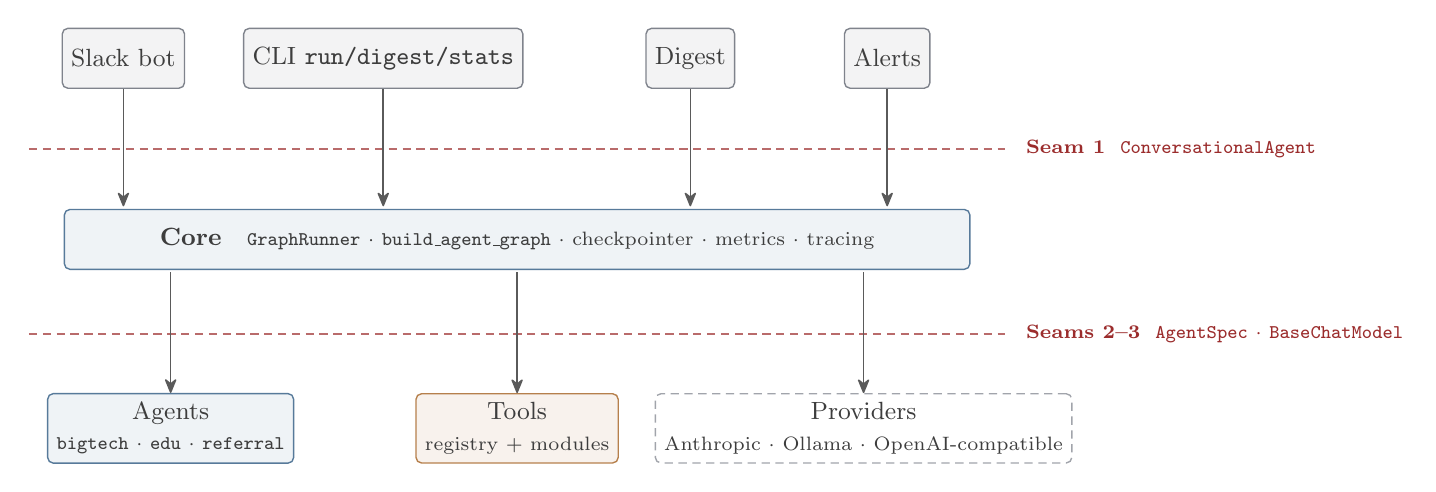
\begin{tikzpicture}[x=1cm,y=1cm]
  \node[infra] (slack)  at (0,2.3)  {Slack bot};
  \node[infra] (cli)    at (3.3,2.3){CLI \texttt{run/digest/stats}};
  \node[infra] (dig)    at (7.2,2.3){Digest};
  \node[infra] (alert)  at (9.7,2.3){Alerts};

  \node[core, minimum width=115mm] (corebox) at (5.0,0)
    {\textbf{Core}\quad\scriptsize \texttt{GraphRunner} $\cdot$ \texttt{build\_\allowbreak{}agent\_\allowbreak{}graph}
     $\cdot$ checkpointer $\cdot$ metrics $\cdot$ tracing};

  \node[core]  (agents) at (0.6,-2.4) {Agents\\\scriptsize \texttt{bigtech} $\cdot$
     \texttt{edu} $\cdot$ \texttt{referral}};
  \node[tool]  (tls)    at (5.0,-2.4) {Tools\\\scriptsize registry $+$ modules};
  \node[ext]   (prov)   at (9.4,-2.4) {Providers\\\scriptsize Anthropic $\cdot$ Ollama $\cdot$
     OpenAI-compatible};

  \draw[draw=cWarn!70, line width=0.9pt, densely dashed] (-1.2,1.15) -- (11.2,1.15);
  \node[faillbl, anchor=west] at (11.4,1.15)
    {\textbf{Seam 1}\ \ \texttt{ConversationalAgent}};
  \draw[draw=cWarn!70, line width=0.9pt, densely dashed] (-1.2,-1.2) -- (11.2,-1.2);
  \node[faillbl, anchor=west] at (11.4,-1.2)
    {\textbf{Seams 2--3}\ \ \texttt{AgentSpec}\ $\cdot$\ \texttt{BaseChatModel}};

  \foreach \n/\x in {slack/0, cli/3.3, dig/7.2, alert/9.7}
    \draw[flow] (\n.south) -- (\x,0.42);
  \foreach \n/\x in {agents/0.6, tls/5.0, prov/9.4}
    \draw[flow] (\x,-0.42) -- (\n.north);
\end{tikzpicture}
\end{adjustbox}
\caption{The three seams. Above the top seam nothing knows what a graph is; below the bottom
seam nothing knows what Slack is. The core is the only layer that has seen both, and it is
the layer that almost never changes.}
\label{fig:seams}
\end{figure}

\begin{description}[leftmargin=0pt,style=nextline,itemsep=3pt]
  \item[Seam 1 --- \texttt{ConversationalAgent} (an ABC).] Everything the Slack adapter is
    allowed to know: \texttt{respond}, \texttt{reset}, \texttt{set\_\allowbreak{}backend},
    \texttt{backend\_\allowbreak{}label}, \texttt{last\_\allowbreak{}backend}, \texttt{tool\_\allowbreak{}names}. It is implemented
    \emph{once}, by \texttt{GraphRunner}, and inherited by both the plain agent and the
    résumé-tailored pipeline --- so the adapter has no branch for ``is this the complicated
    one''.
  \item[Seam 2 --- \texttt{AgentSpec} (a dataclass).] An agent is declared, not coded: key,
    display name, system prompt, tool modules, default backend, and the two behaviour flags.
    The rule that makes the seam real is that adding an agent must never edit the graph.
  \item[Seam 3 --- the LangChain chat model.] One builder per provider behind
    \texttt{BaseChatModel}. The consequence reaches much further than provider swapping:
    because history is stored as provider-agnostic message objects rather than as any
    vendor's wire format, a user can change model in the middle of a conversation and the
    thread replays cleanly into the new provider.
\end{description}

\begin{table}[!ht]
\centering\tablefont
\caption{Change surface. The test of the layering is not how the diagram looks but how
small the diff is for each routine change.}
\label{tab:blast}
\begin{tabularx}{\textwidth}{L{4.1cm} X L{3.0cm}}
\toprule
\textbf{Change} & \textbf{What it touches} & \textbf{Never touches} \\
\midrule
Add an agent & one file in \texttt{scout/agents/}, one line in \texttt{AGENTS} & the graph,
  the Slack layer \\
Add a tool & one module with \texttt{register(reg)}, one entry in a spec's
  \texttt{tool\_\allowbreak{}modules} & the registry, the graph \\
Add a job source & one module under \texttt{tools/jobs/}, one line in
  \texttt{directory.SOURCES} & the shared HTTP, render and relevance code \\
Add a company on an existing platform & one line in that platform's \texttt{BOARDS} (it
  reaches the referral directory on its own) & everything else \\
Add a model provider & one builder, one entry in \texttt{\_\allowbreak{}BUILDERS} & agents, tools,
  history \\
Add a daily digest & set \texttt{in\_\allowbreak{}digest} on the spec, add one systemd timer &
  \texttt{scout/digest.py} \\
\bottomrule
\end{tabularx}
\end{table}

% ==========================================================================
\section{The two graphs}
% ==========================================================================

Every agent compiles to the same model/tool loop (Figure~\ref{fig:loop}). Agents that opt
into résumé tailoring are wrapped in a second, outer graph (Figure~\ref{fig:orch}).

\begin{figure}[!ht]
\centering
\begin{adjustbox}{max width=\textwidth}
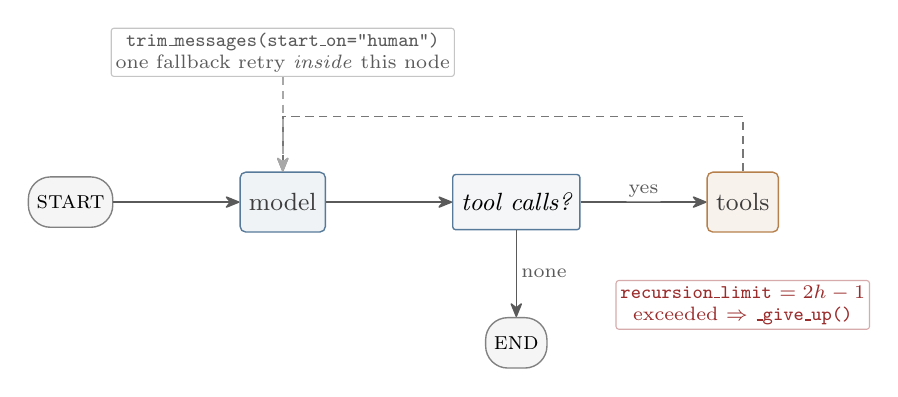
\begin{tikzpicture}[node distance=9mm and 16mm]
  \node[term] (start) {start};
  \node[core, right=of start] (model) {model};
  \node[dec, right=of model] (cond) {tool calls?};
  \node[tool, right=of cond] (tools) {tools};
  \node[term, below=11mm of cond] (end) {end};

  \draw[flow] (start) -- (model);
  \draw[flow] (model) -- (cond);
  \draw[flow] (cond) -- node[lbl,above]{yes} (tools);
  \draw[flow] (cond) -- node[lbl,right]{none} (end);
  \draw[back] (tools.north) -- ++(0,7mm) -| (model.north);

  \node[lbl, above=12mm of model, align=center, draw=cEdge!30]
    {\texttt{trim\_\allowbreak{}messages(start\_\allowbreak{}on="human")}\\one fallback retry \emph{inside} this node};
  \draw[back, draw=cEdge!45] ([yshift=12mm]model.north) -- (model.north);

  \node[lbl, below=6mm of tools, align=center, draw=cWarn!40, text=cWarn]
    {\texttt{recursion\_\allowbreak{}limit} $= 2h-1$\\exceeded $\Rightarrow$ \texttt{\_\allowbreak{}give\_\allowbreak{}up()}};
\end{tikzpicture}
\end{adjustbox}
\caption{The shared agent graph. Three mechanisms hang off it, and each is deliberately
placed \emph{in} a node rather than around the turn: window trimming and the fallback retry
live in the model node, and the hop limit is expressed as LangGraph's recursion limit.}
\label{fig:loop}
\end{figure}

\paragraph{Window trimming is load-bearing.} The tail of the conversation is selected with
\texttt{trim\_\allowbreak{}messages(..., start\_\allowbreak{}on="human")}. That argument is not cosmetic: providers
reject a conversation that opens on the assistant's side, and a tool result must never lead
the window or be separated from the tool call it answers. Because tool traffic is
checkpointed --- unlike the hand-rolled loop this replaced, where it was per-turn --- the
model remembers what it already looked up, at the cost of a shorter reach back through a
tool-heavy conversation.

\paragraph{The hop limit is arithmetic, not a guess.} A tool hop is two LangGraph
super-steps (model, then tools) and a turn always ends on a model step, so $h$ hops is
$2h-1$ steps. Exceeding it raises \texttt{GraphRecursionError}, which is handled rather than
propagated (\S\ref{sec:failure}).

\begin{figure}[!ht]
\centering
\begin{adjustbox}{max width=\textwidth}
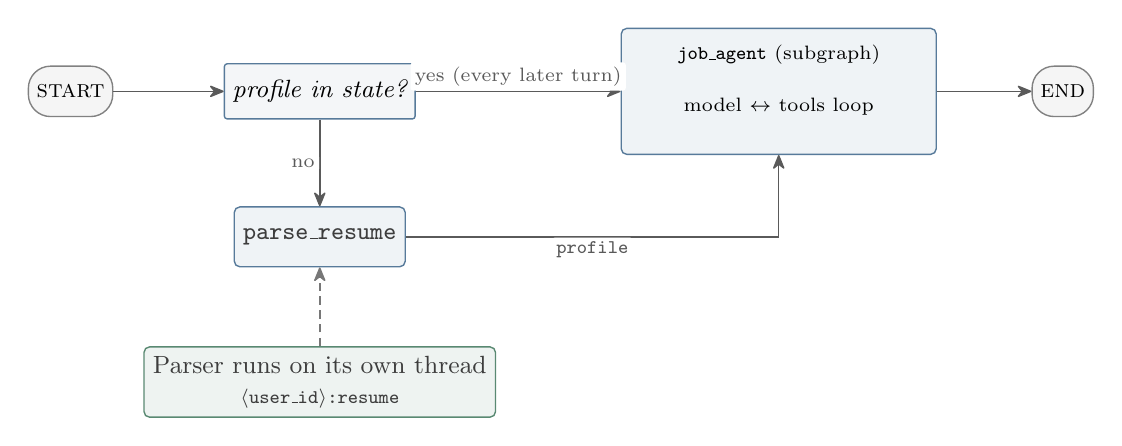
\begin{tikzpicture}[node distance=9mm and 14mm]
  \node[term] (start) {start};
  \node[dec, right=of start] (router) {profile in state?};
  \node[core, below=11mm of router] (parse) {\texttt{parse\_\allowbreak{}resume}};
  \node[core, right=26mm of router, minimum width=40mm, minimum height=16mm] (job) {\ };
  \node[anchor=north] at ([yshift=-1mm]job.north) {\scriptsize\textbf{\texttt{job\_\allowbreak{}agent}}
    (subgraph)};
  \node[font=\scriptsize] at ([yshift=-2mm]job.center) {model $\leftrightarrow$ tools loop};
  \node[term, right=12mm of job] (end) {end};

  \draw[flow] (start) -- (router);
  \draw[flow] (router) -- node[lbl,above]{yes (every later turn)} (job);
  \draw[flow] (router) -- node[lbl,left]{no} (parse);
  \draw[flow] (parse.east) -| node[lbl,pos=0.25,below]{\texttt{profile}} (job.south);
  \draw[flow] (job) -- (end);

  \node[state, below=10mm of parse, align=center] (pth)
    {Parser runs on its own thread\\\scriptsize\texttt{$\langle$user\_\allowbreak{}id$\rangle$:resume}};
  \draw[back] (pth) -- (parse);
\end{tikzpicture}
\end{adjustbox}
\caption{The résumé-tailored orchestration graph. The router reads the profile out of
checkpointed graph state, so the cache \emph{is} the state --- not a dictionary kept beside
it. The parser's own tool calls and JSON reply never enter the job agent's history; only the
rendered brief crosses, appended to the job agent's system prompt.}
\label{fig:orch}
\end{figure}

Three properties follow from putting the cache in graph state rather than in a Python
dictionary. It survives a restart whenever \texttt{CHECKPOINT\_\allowbreak{}DB} is set, so a deployed bot
parses a résumé once rather than once per restart. It is dropped by
\texttt{-{}-reset} along with the thread, which is exactly the behaviour a user expects
after editing their résumé. And it needs no invalidation logic, because there is no second
place for it to go stale in.

One subtlety worth knowing before an interviewer finds it: a subgraph is handed the
recursion limit \emph{afresh}, so the outer graph's extra nodes raise a \emph{floor}
(\texttt{\_\allowbreak{}min\_\allowbreak{}steps}) rather than adding to the limit. Adding would silently hand the
inner tool loop extra hops.

% ==========================================================================
\section{The life of a message}
% ==========================================================================

Figure~\ref{fig:seq} traces one DM end to end. The ordering of three steps matters more
than the rest: the per-user lock is taken before anything else, the traced config is a
\emph{copy}, and metrics are recorded after the reply is known but inside the lock.

\begin{figure}[!ht]
\centering
\begin{adjustbox}{max width=\textwidth}
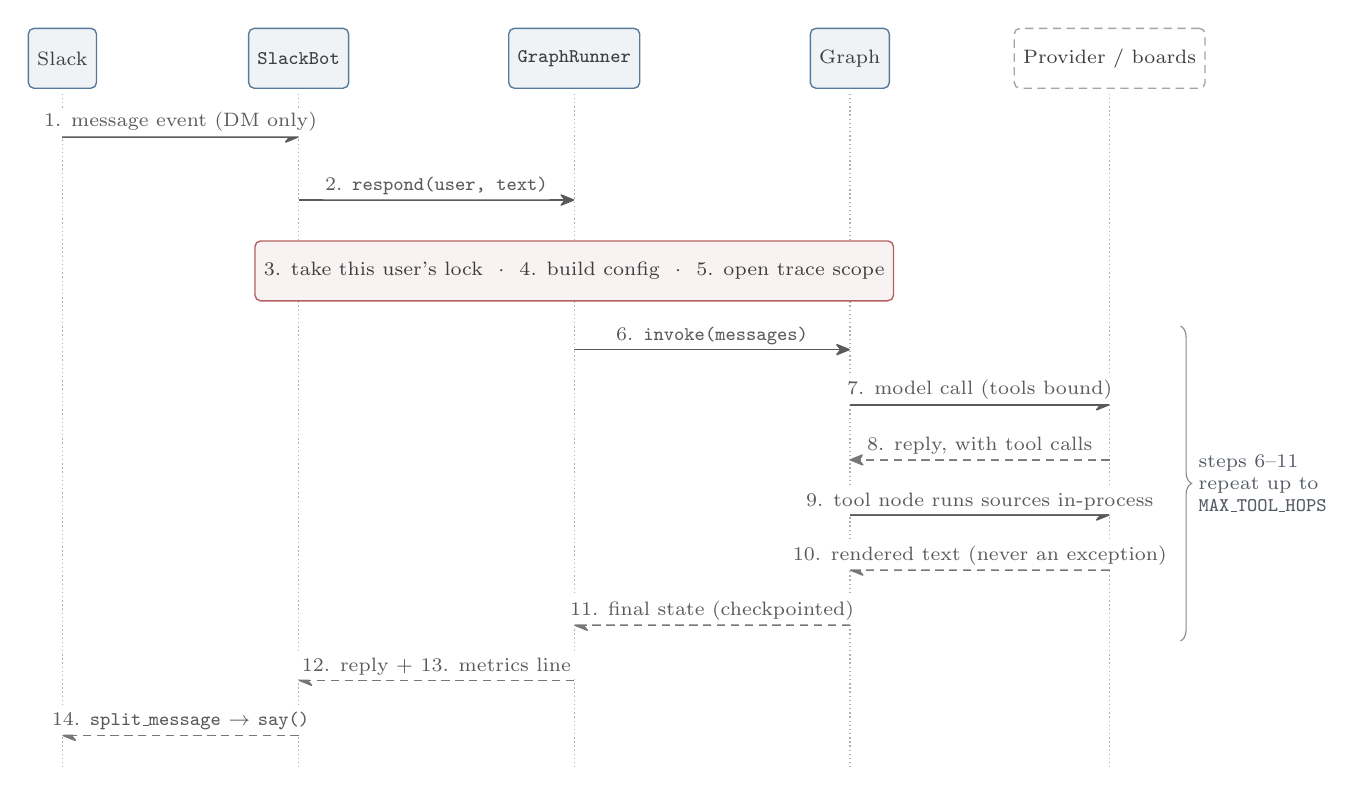
\begin{tikzpicture}[font=\small,x=1cm,y=1cm]
  \def\lifeA{0}\def\lifeB{3.0}\def\lifeC{6.5}\def\lifeD{10.0}\def\lifeE{13.3}
  \def\bottom{-9.0}

  \node[core] (A) at (\lifeA,0) {\scriptsize Slack};
  \node[core] (B) at (\lifeB,0) {\scriptsize \texttt{SlackBot}};
  \node[core] (C) at (\lifeC,0) {\scriptsize \texttt{GraphRunner}};
  \node[core] (D) at (\lifeD,0) {\scriptsize Graph};
  \node[ext]  (E) at (\lifeE,0) {\scriptsize Provider / boards};

  \foreach \x in {\lifeA,\lifeB,\lifeC,\lifeD,\lifeE}
    \draw[life] (\x,-0.45) -- (\x,\bottom);

  \draw[flow] (\lifeA,-1.0) -- (\lifeB,-1.0)
    node[lbl,midway,above]{\scriptsize 1. message event (DM only)};
  \draw[flow] (\lifeB,-1.8) -- (\lifeC,-1.8)
    node[lbl,midway,above]{\scriptsize 2. \texttt{respond(user, text)}};
  \node[warn, minimum width=52mm, font=\scriptsize] at (\lifeC,-2.7)
    {3. take this user's lock \ $\cdot$ \ 4. build config \ $\cdot$ \ 5. open trace scope};
  \draw[flow] (\lifeC,-3.7) -- (\lifeD,-3.7)
    node[lbl,midway,above]{\scriptsize 6. \texttt{invoke(messages)}};
  \draw[flow] (\lifeD,-4.4) -- (\lifeE,-4.4)
    node[lbl,midway,above]{\scriptsize 7. model call (tools bound)};
  \draw[back] (\lifeE,-5.1) -- (\lifeD,-5.1)
    node[lbl,midway,above]{\scriptsize 8. reply, with tool calls};
  \draw[flow] (\lifeD,-5.8) -- (\lifeE,-5.8)
    node[lbl,midway,above]{\scriptsize 9. tool node runs sources in-process};
  \draw[back] (\lifeE,-6.5) -- (\lifeD,-6.5)
    node[lbl,midway,above]{\scriptsize 10. rendered text (never an exception)};
  \draw[back] (\lifeD,-7.2) -- (\lifeC,-7.2)
    node[lbl,midway,above]{\scriptsize 11. final state (checkpointed)};
  \draw[back] (\lifeC,-7.9) -- (\lifeB,-7.9)
    node[lbl,midway,above]{\scriptsize 12. reply $+$ 13. metrics line};
  \draw[back] (\lifeB,-8.6) -- (\lifeA,-8.6)
    node[lbl,midway,above]{\scriptsize 14. \texttt{split\_\allowbreak{}message} $\rightarrow$ \texttt{say()}};

  \draw[decorate,decoration={brace,amplitude=4pt},draw=cInfra!70]
    (14.2,-3.4) -- (14.2,-7.4)
    node[midway,right=3pt,font=\scriptsize,text=cInfra,align=left]
    {steps 6--11\\repeat up to\\\texttt{MAX\_\allowbreak{}TOOL\_\allowbreak{}HOPS}};
\end{tikzpicture}
\end{adjustbox}
\caption{One turn, end to end. Steps 6--11 are the loop of Figure~\ref{fig:loop}; everything
outside them happens exactly once per message. Step 9 runs tools in-process --- the tool node
is Python, not a service call --- which is why a tool must return a sentence rather than
raise.}
\label{fig:seq}
\end{figure}

\paragraph{The lock.} \texttt{slack-bolt} dispatches events on a thread pool, so two
messages from the same user can arrive concurrently and interleave into one thread. One
\texttt{RLock} per user serialises that user's turns while different users still run in
parallel --- the granularity that matters, given that a turn can take tens of seconds.

\paragraph{Why the traced config is a copy.} \texttt{GraphRunner.\_\allowbreak{}config} returns an
\emph{untraced} config, because that same config is used for checkpointer reads and for the
repair written after a stuck turn, neither of which is part of the turn a human would want
to read in a trace. \texttt{tracing.traced} yields a new dictionary with the callback added.
Nothing in the graph branches on whether a turn is observed.

% ==========================================================================
\section{The job-source subsystem}
% ==========================================================================

Sixteen source modules cover 29 companies. They are organised along two axes at once
(Figure~\ref{fig:sources}): by \emph{platform}, which is how an implementation has to be
organised, and by \emph{company}, which is how a user thinks.

\begin{figure}[!ht]
\centering
\begin{adjustbox}{max width=\textwidth}
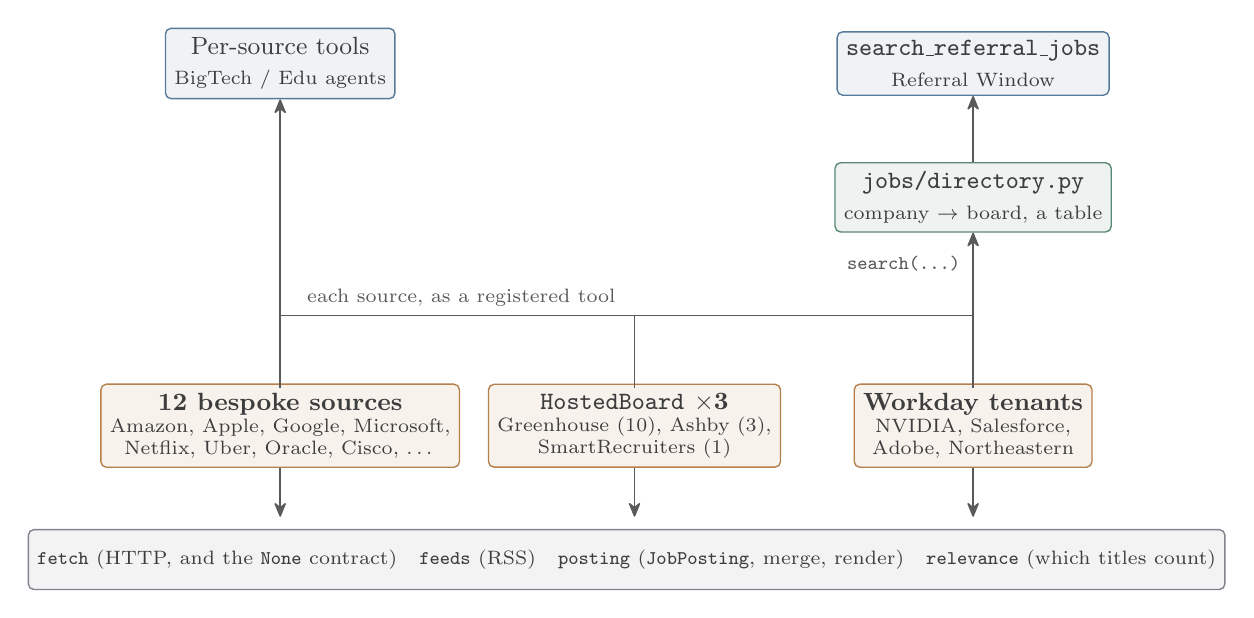
\begin{tikzpicture}[x=1cm,y=1cm]
  \node[core] (agenttools) at (1.6,0.7)  {Per-source tools\\\scriptsize BigTech / Edu agents};
  \node[core] (refsearch)  at (10.4,0.7)  {\texttt{search\_\allowbreak{}referral\_\allowbreak{}jobs}\\\scriptsize Referral Window};
  \node[state](dir)        at (10.4,-1.0) {\texttt{jobs/directory.py}\\\scriptsize company $\rightarrow$ board, a table};

  \node[tool, font=\scriptsize, align=center] (bespoke) at (1.6,-3.9)
    {\textbf{\small 12 bespoke sources}\\Amazon, Apple, Google, Microsoft,\\Netflix, Uber, Oracle, Cisco, \dots};
  \node[tool, font=\scriptsize, align=center] (hosted) at (6.1,-3.9)
    {\textbf{\small \texttt{HostedBoard} $\times$3}\\Greenhouse (10), Ashby (3),\\SmartRecruiters (1)};
  \node[tool, font=\scriptsize, align=center] (wd) at (10.4,-3.9)
    {\textbf{\small Workday tenants}\\NVIDIA, Salesforce,\\Adobe, Northeastern};

  \node[infra, minimum width=118mm, font=\scriptsize] (shared) at (6.0,-5.6)
    {\texttt{fetch} (HTTP, and the \texttt{None} contract)\quad \texttt{feeds} (RSS)\quad
     \texttt{posting} (\texttt{JobPosting}, merge, render)\quad \texttt{relevance} (which titles count)};

  % the shared bus above the sources
  \draw[draw=cEdge!85, line width=0.55pt] (1.6,-2.5) -- (10.4,-2.5);
  \foreach \x in {1.6,6.1,10.4} \draw[draw=cEdge!85, line width=0.55pt] (\x,-3.42) -- (\x,-2.5);
  \draw[flow] (1.6,-2.5) -- (agenttools.south);
  \draw[flow] (10.4,-2.5) -- (dir.south);
  \draw[flow] (dir) -- (refsearch);
  \node[lbl, anchor=south] at (3.9,-2.45) {\scriptsize each source, as a registered tool};
  \node[lbl, anchor=south east] at (10.3,-2.0) {\scriptsize \texttt{search(...)}};

  \foreach \n in {bespoke,hosted,wd} \draw[flow] (\n.south) -- ++(0,-0.62);
\end{tikzpicture}
\end{adjustbox}
\caption{Two indexes over one set of sources. Upward-left: every source is a registered tool a
job agent calls by name. Upward-right: every source is also a plain \texttt{search(...)}
function, which \texttt{directory.py} indexes \emph{by company} so the Referral Window can
sweep a list of employers rather than a list of tools. Everything rests on one shared layer.}
\label{fig:sources}
\end{figure}

\paragraph{Every source exposes its search twice.} A registered tool returning Slack text,
and a \texttt{search(keywords, limit) -> list[JobPosting] | None} matching a
\texttt{Searcher} protocol, of which the tool is a thin renderer. The second form is what
lets one caller search many companies and merge the results; without it, the Referral Window
would have to drive a dozen tools and re-parse their prose.

\paragraph{\texttt{None} is not \texttt{[]}.} Every fetch helper returns \texttt{None} for
any failure whatsoever --- connection refused, HTTP 500, a body that will not decode --- and
that \texttt{None} propagates all the way to the reply as ``I could not look''. An empty list
means ``I looked, and there is nothing''. Collapsing the two is the one failure mode that
sends someone away from a company they should have asked, and it is the single contract
every source in the system is written against.

\paragraph{A keyword box is not a title filter.} Several boards match the query against the
whole posting, so searching ``machine learning'' returns account executives whose
description mentions it. Every title is therefore re-gated through
\texttt{relevance.is\_\allowbreak{}ai\_\allowbreak{}ml\_\allowbreak{}role} after the source returns, and when the model supplies no
keywords the module falls back to five profile queries merged and de-duplicated.

\begin{table}[!ht]
\centering\tablefont
\caption{The sixteen source modules and what each had to work around. ``Date'' records
whether the source publishes a real timestamp; where it does not, the source's own wording
is carried verbatim in \texttt{posted\_\allowbreak{}label} and never coerced into a date.}
\label{tab:sources}
\begin{tabularx}{\textwidth}{L{2.6cm} L{3.0cm} c X}
\toprule
\textbf{Source} & \textbf{Mechanism} & \textbf{Date} & \textbf{The awkward part} \\
\midrule
Amazon & JSON endpoint & yes & No relevance filter; each profile query is run and merged. \\
Apple & server-rendered page & yes & The documented search API needs a CSRF token; the page's
  own embedded state is read instead. \\
Google & HTML scrape & no & No API and no dates, so the site's own ordering is kept. \\
Microsoft & Eightfold JSON & yes & Rows are buried under \texttt{data}; the old careers API
  is gone. \\
Netflix & Eightfold JSON & yes & Keyword, location and recency filtering are all server-side. \\
Uber & JSON board & yes & One request returns the whole US board. \\
Oracle & Oracle Cloud Recruiting & yes & Rows sit under \texttt{items[0]}; a missing key means
  \emph{unreachable}, not empty. \\
Cisco & Phenom widget POST & yes & Rows under \texttt{refineSearch.data}. \\
Bloomberg & Avature scrape & no & \texttt{careers.bloomberg.com} is a redirect dead end;
  nothing is published. \\
Lenovo & Avature RSS & label & Feed carries relative wording only. \\
Boston University & SilkRoad RSS & label & No search API at all. \\
Greenhouse & \texttt{HostedBoard} & yes & 10 companies, one shape; no server-side filtering. \\
Ashby & \texttt{HostedBoard} & yes & 3 companies, same shape. \\
SmartRecruiters & \texttt{HostedBoard} & yes & 1 company; country field double-checked. \\
Workday & CXS POST & label & 3 tenants; 20-row page cap, and an out-of-range offset
  \emph{wraps} to page one, so paging cannot terminate. \\
Northeastern & Workday CXS & label & Same platform, different tenant shape. \\
\bottomrule
\end{tabularx}
\end{table}

\paragraph{One shape, written once.} Greenhouse, Ashby and SmartRecruiters are not three
sources; they are one shape written three times --- a board per company at a predictable URL,
no server-side filtering, one JSON row per opening. \texttt{HostedBoard} holds that shape
(slug lookup, fetch, title filtering, and the three answers such a tool must tell apart:
company we do not host, board that was down, board with nothing matching). A platform module
supplies only what differs: where its boards live and how to read one row. Workday is
deliberately \emph{not} folded into it: it takes a POST body rather than a slug in a path,
and its URL needs three parts rather than one. Nothing about the two lines up, so forcing
them together would produce an abstraction that is harder to read than either.

% ==========================================================================
\section{Decision log}
% ==========================================================================

Table~\ref{tab:decisions} is the short form of every decision that shaped the system, with
what it cost. The four expanded below are the ones whose reasoning is least obvious from the
code.

\begin{table}[!ht]
\centering\tablefont
\caption{Decision log. A decision with no cost in the right-hand column is usually a
decision that has not been thought about.}
\label{tab:decisions}
\begin{tabularx}{\textwidth}{L{0.4cm} L{3.5cm} L{3.0cm} X L{3.1cm}}
\toprule
\textbf{\#} & \textbf{Decision} & \textbf{Rejected} & \textbf{Why} & \textbf{What it costs} \\
\midrule
1 & LangGraph, not a hand-rolled tool loop & keep the bespoke \texttt{while} loop &
  Checkpointing, subgraphs and a tool node arrive for free; tool traffic becomes part of
  history, so the model remembers what it looked up &
  Tool messages consume the \texttt{MAX\_\allowbreak{}TURNS} window \\
2 & History \emph{is} the checkpointer thread, keyed by Slack user id & an application-level
  message list & Provider-agnostic replay, model switching mid-conversation,
  \texttt{-{}-reset} is a thread delete & Two bots on one database file share a thread
  unless each gets its own path \\
3 & Résumé profile cached in graph state & a dictionary beside the graph & Survives
  restarts, needs no invalidation logic, dropped with the thread & A changed résumé needs
  an explicit \texttt{-{}-reset} \\
4 & \texttt{None} $\neq$ \texttt{[]} in every source & return \texttt{[]} on failure &
  Makes a completeness claim possible at all & Every source and every caller must carry the
  distinction \\
5 & Company-to-board routing is a table & let the model route by name & The Referral Window
  can name what it could \emph{not} check & The table is maintained by hand \\
6 & Referral list outside the checkpointer & store it with history & User-typed data
  survives \texttt{-{}-reset} and redeploy & A second store, with its own locking and
  atomic write \\
7 & Split capability: \texttt{referrals\_\allowbreak{}read} vs \texttt{referrals} & one tool module for
  both & A searching agent cannot mutate the list & Two modules instead of one \\
8 & One process per agent, one Slack token & one process hosting every agent & Each
  digest lands in its own DM window & Three resident processes on 916\,MB \\
9 & Model retry \emph{inside} the model node & retry around the whole turn & A node that
  raises commits nothing, so the retry starts clean but keeps tool results already fetched &
  The fallback must be a working backend, or every failure fails twice \\
10 & Tools return sentences, never raise & let exceptions propagate & One dead board cannot
  fail a whole turn & A real bug can hide behind a polite message \\
11 & Observability added to a \emph{config}, never a code path & instrument the graph &
  No branch anywhere knows whether a turn is traced & The root span must be owned explicitly
  to make the trace's input/output the question and the answer \\
12 & Digest membership derived from \texttt{in\_\allowbreak{}digest} & a registry beside \texttt{AGENTS} &
  A new job agent joins the digest by existing & Each one still needs its own systemd timer \\
13 & \texttt{settings.py} never raises on import & validate configuration at import &
  The package stays importable and testable with no \texttt{.env} & Validation must be
  called explicitly at each entry point \\
\bottomrule
\end{tabularx}
\end{table}

\subsection{Why the retry lives in the model node (\#9)}

The obvious place to retry a failed model call is around the turn: catch, switch backend,
run the turn again. That is wrong here for a reason specific to graphs. A LangGraph node
that raises commits nothing to state, so retrying \emph{inside} the node starts from a clean
slate --- no half-written assistant message, no orphaned tool call --- while every tool
result the turn has already fetched is still in state and is not re-fetched. Retrying around
the turn would either discard that work or replay it, and replaying means hitting a dozen
careers boards a second time. Three tests pin the behaviour:
\texttt{test\_\allowbreak{}failed\_\allowbreak{}call\_\allowbreak{}is\_\allowbreak{}retried\_\allowbreak{}on\_\allowbreak{}the\_\allowbreak{}fallback},
\texttt{test\_\allowbreak{}fallback\_\allowbreak{}sees\_\allowbreak{}no\_\allowbreak{}trace\_\allowbreak{}of\_\allowbreak{}the\_\allowbreak{}failed\_\allowbreak{}attempt}, and
\texttt{test\_\allowbreak{}tool\_\allowbreak{}results\_\allowbreak{}already\_\allowbreak{}fetched\_\allowbreak{}survive\_\allowbreak{}the\_\allowbreak{}fallback}.

The fallback is disclosed to the user rather than applied silently, because a local 3B model
and Claude differ enough that a silent swap would be misleading. An empty
\texttt{FALLBACK\_\allowbreak{}BACKEND} disables the retry entirely, which is what a container with no
Ollama in it needs --- otherwise every Claude failure fails twice, slowly.

\subsection{Why one process holds exactly one agent (\#8)}

A process holds one Slack bot token. An earlier version ran all digests in one process,
which meant every agent's morning report was posted by whichever app was the default ---
three reports stacked in one conversation, attributed to the wrong bot. Splitting them is
not a scaling decision; it is an identity one. The systemd template unit makes the split
nearly free (\S\ref{sec:deploy}): \texttt{scout@bigtech} and \texttt{scout@edu} are the same
unit file instantiated twice, each reading its own \texttt{EnvironmentFile}. The cost is
memory --- three resident Python processes plus three periodic ones on a 916\,MB box with no
swap --- which is why the digest timers are staggered ten minutes apart rather than fired
together.

\subsection{Why the referral list is not checkpointed (\#6)}

History is disposable. It is trimmed on every turn, it is deleted by \texttt{-{}-reset}, and
losing it costs the user nothing they would notice. The referral list is the opposite: a
handful of companies the user typed once and expects to find again, and the thing that makes
one agent's answer worth reading. Putting it in the checkpointer would couple its lifetime to
history's, so a reset --- something a user does casually --- would silently delete it.

It is therefore a JSON document in \texttt{state/}, rewritten whole under a lock, written to
a temporary file and renamed so a crash mid-write leaves the previous list intact rather than
a truncated file. A file that will not parse raises rather than silently starting over: the
file is the user's data, and a bad parse is far more likely to be a bug than a real reset.
\texttt{deploy.sh} excludes \texttt{state/} from its rsync, so a redeploy cannot overwrite
the box's list with whatever happens to be on a laptop.

\subsection{Why capability is split rather than prompted (\#7)}

The job agents are told in their system prompt never to edit the referral list. That
instruction is real, and it is not the mechanism. The mechanism is that
\texttt{add\_\allowbreak{}referral} and \texttt{remove\_\allowbreak{}referral} are not in their tool set at all: they
import \texttt{referrals\_\allowbreak{}read}, which registers only \texttt{list\_\allowbreak{}referrals}. An agent that
searches twelve boards and ranks the results will, often enough to matter, decide that
recording something would be helpful --- and the user never asked it to.

The same principle runs the other way for the Referral Window, which \emph{may} write. What
makes that safe is that its only search tool is \texttt{search\_\allowbreak{}referral\_\allowbreak{}jobs}, which takes
the list as its scope; there is nothing in its tool set to search with off-list. The
invariant is guarded directly by
\texttt{test\_\allowbreak{}the\_\allowbreak{}referral\_\allowbreak{}window\_\allowbreak{}can\_\allowbreak{}only\_\allowbreak{}search\_\allowbreak{}within\_\allowbreak{}the\_\allowbreak{}list}.

Related, and worth stating because it surprises people: a tool that needs to know \emph{who}
is asking declares \texttt{*, config: RunnableConfig}. LangChain injects it and hides it from
the schema the model sees, so the model is never asked to supply a user id and therefore
cannot get one wrong. The annotation must stay exactly \texttt{RunnableConfig} --- widening
it to \texttt{RunnableConfig | None} stops LangChain recognising it, the injection silently
stops, and \texttt{config} reappears as a parameter the model is asked to fill.
\texttt{test\_\allowbreak{}the\_\allowbreak{}user\_\allowbreak{}id\_\allowbreak{}is\_\allowbreak{}not\_\allowbreak{}in\_\allowbreak{}the\_\allowbreak{}schema\_\allowbreak{}the\_\allowbreak{}model\_\allowbreak{}sees} guards it.

% ==========================================================================
\section{Failure modes}
\label{sec:failure}
% ==========================================================================

Every external dependency in this system is somebody else's website. Degradation is
therefore the normal case, not the exceptional one, and each mode has a designed response
(Figure~\ref{fig:failure}, Table~\ref{tab:failures}).

\begin{figure}[!ht]
\centering
\begin{adjustbox}{max width=\textwidth}
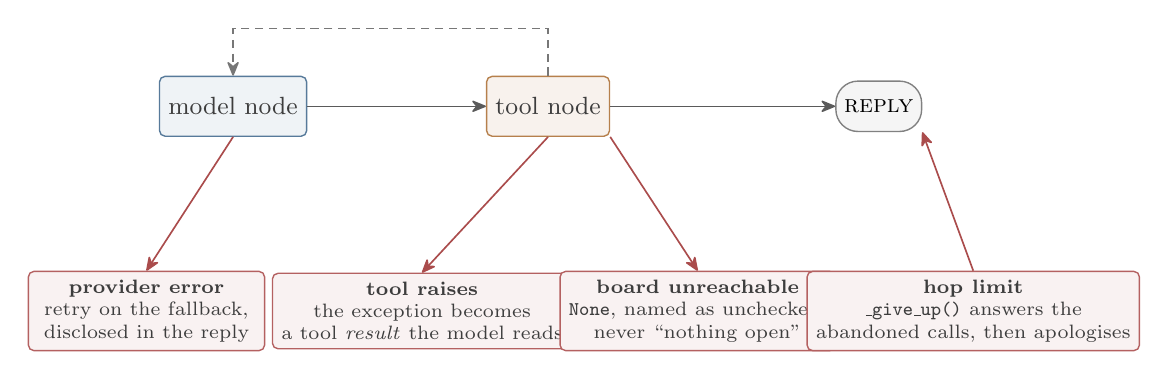
\begin{tikzpicture}[x=1cm,y=1cm]
  \node[core] (model) at (2.2,0)  {model node};
  \node[tool] (tools) at (6.2,0)  {tool node};
  \node[term] (reply) at (10.4,0) {reply};

  \draw[flow] (model) -- (tools);
  \draw[flow] (tools) -- (reply);
  \draw[back] (tools.north) -- ++(0,0.6) -| (model.north);

  \node[warn, minimum width=30mm, font=\scriptsize, align=center] (c1) at (1.1,-2.6)
    {\textbf{provider error}\\\scriptsize retry on the fallback,\\\scriptsize disclosed in the reply};
  \node[warn, minimum width=30mm, font=\scriptsize, align=center] (c2) at (4.6,-2.6)
    {\textbf{tool raises}\\\scriptsize the exception becomes\\\scriptsize a tool \emph{result} the model reads};
  \node[warn, minimum width=30mm, font=\scriptsize, align=center] (c3) at (8.1,-2.6)
    {\textbf{board unreachable}\\\scriptsize \texttt{None}, named as unchecked,\\\scriptsize never ``nothing open''};
  \node[warn, minimum width=30mm, font=\scriptsize, align=center] (c4) at (11.6,-2.6)
    {\textbf{hop limit}\\\scriptsize \texttt{\_\allowbreak{}give\_\allowbreak{}up()} answers the\\\scriptsize abandoned calls, then apologises};

  \draw[fail] (model.south) -- (c1.north);
  \draw[fail] (tools.south) -- (c2.north);
  \draw[fail] (tools.south east) -- (c3.north);
  \draw[fail] (c4.north) -- (reply.south east);
\end{tikzpicture}
\end{adjustbox}
\caption{Failure paths, in red. None of them terminates the turn: a failed provider is retried
on another, a raised tool becomes text the model can act on, an unreachable board is reported
as unchecked rather than empty, and a turn that exhausts its hops repairs its own thread
before apologising.}
\label{fig:failure}
\end{figure}

\begin{table}[!ht]
\centering\tablefont
\caption{Failure modes and their designed responses. Every row has a test, because a
degradation path that is not tested is a degradation path that does not work.}
\label{tab:failures}
\begin{tabularx}{\textwidth}{L{3.1cm} L{2.9cm} X L{3.4cm}}
\toprule
\textbf{Failure} & \textbf{Detected by} & \textbf{Response} & \textbf{Guarded by} \\
\midrule
Provider request fails & exception in the model node & Retry once on
  \texttt{FALLBACK\_\allowbreak{}BACKEND} within the same turn; the reply says which model answered &
  \texttt{test\_\allowbreak{}failed\_\allowbreak{}call\_\allowbreak{}is\_\allowbreak{}retried\_\allowbreak{}on\_\allowbreak{}the\_\allowbreak{}fallback} \\
No fallback configured & \texttt{FALLBACK\_\allowbreak{}BACKEND} empty or unknown & Raise, so the Slack
  layer reports it rather than failing twice slowly &
  \texttt{test\_\allowbreak{}an\_\allowbreak{}empty\_\allowbreak{}fallback\_\allowbreak{}setting\_\allowbreak{}disables\_\allowbreak{}the\_\allowbreak{}retry} \\
A tool raises & \texttt{ToolNode(handle\_\allowbreak{}tool\_\allowbreak{}errors=...)} & The exception is turned into a
  tool result the model reads and can act on &
  \texttt{test\_\allowbreak{}failing\_\allowbreak{}tool\_\allowbreak{}becomes\_\allowbreak{}a\_\allowbreak{}message\_\allowbreak{}for\_\allowbreak{}the\_\allowbreak{}model} \\
Model invents a tool name & LangGraph & Reported back to the model as a result, not an error &
  \texttt{test\_\allowbreak{}unknown\_\allowbreak{}tool\_\allowbreak{}is\_\allowbreak{}reported\_\allowbreak{}to\_\allowbreak{}the\_\allowbreak{}model} \\
Hop limit exhausted & \texttt{GraphRecursionError} & \texttt{\_\allowbreak{}give\_\allowbreak{}up()} answers every
  abandoned tool call, \emph{then} records the apology, so the thread stays valid &
  \texttt{test\_\allowbreak{}thread\_\allowbreak{}survives\_\allowbreak{}the\_\allowbreak{}hop\_\allowbreak{}limit} \\
Job board unreachable & \texttt{fetch} returns \texttt{None} & Named in the reply as
  unchecked; never merged into ``nothing found'' &
  \texttt{test\_\allowbreak{}an\_\allowbreak{}unreachable\_\allowbreak{}board\_\allowbreak{}is\_\allowbreak{}named\_\allowbreak{}not\_\allowbreak{}read\_\allowbreak{}as\_\allowbreak{}empty} \\
Every board down & all searches \texttt{None} & A different sentence again: ``could not
  reach any of them'' &
  \texttt{test\_\allowbreak{}every\_\allowbreak{}board\_\allowbreak{}being\_\allowbreak{}down\_\allowbreak{}is\_\allowbreak{}not\_\allowbreak{}reported\_\allowbreak{}as\_\allowbreak{}nothing\_\allowbreak{}open} \\
Company has no board & \texttt{directory.resolve} returns \texttt{None} & Listed as a
  coverage gap the user must check themselves &
  \texttt{test\_\allowbreak{}a\_\allowbreak{}company\_\allowbreak{}with\_\allowbreak{}no\_\allowbreak{}board\_\allowbreak{}is\_\allowbreak{}named\_\allowbreak{}too} \\
Referral store corrupt & JSON decode error & Refuse to read, answer in words; never silently
  start a fresh list & \texttt{test\_\allowbreak{}an\_\allowbreak{}unreadable\_\allowbreak{}store\_\allowbreak{}answers\_\allowbreak{}in\_\allowbreak{}words} \\
Model returns nothing & empty reply text & Substitute a readable message rather than sending
  an empty Slack post & \texttt{test\_\allowbreak{}empty\_\allowbreak{}reply\_\allowbreak{}becomes\_\allowbreak{}something\_\allowbreak{}readable} \\
Résumé file unreadable & parse failure & Name the file instead of raising; the search
  degrades to untailored & \texttt{test\_\allowbreak{}a\_\allowbreak{}corrupt\_\allowbreak{}file\_\allowbreak{}names\_\allowbreak{}the\_\allowbreak{}file\_\allowbreak{}instead\_\allowbreak{}of\_\allowbreak{}raising} \\
Langfuse will not start & exception building the client & Log once, run untraced for the life
  of the process & \texttt{test\_\allowbreak{}a\_\allowbreak{}turn\_\allowbreak{}still\_\allowbreak{}answers\_\allowbreak{}when\_\allowbreak{}tracing\_\allowbreak{}will\_\allowbreak{}not\_\allowbreak{}start} \\
Unit exceeds its restart burst & systemd \texttt{OnFailure=} & \texttt{scout-alert@} DMs the
  last 20 journal lines & \texttt{tests/test\_\allowbreak{}alert.py} \\
\bottomrule
\end{tabularx}
\end{table}

\paragraph{The repair is the interesting one.} When a turn runs out of tool hops, the run
stops with tool calls still unanswered. Every provider rejects a conversation in which a tool
request has no result, so simply apologising would leave a thread that breaks the user's
\emph{next} message, not just this one. \texttt{\_\allowbreak{}give\_\allowbreak{}up()} therefore writes a synthetic
result for each abandoned call before recording the apology. It is a one-screen method and
it is the difference between one bad turn and a conversation that has to be reset.

% ==========================================================================
\section{Concurrency and state}
% ==========================================================================

Four things are stored, in three places, with three different lifetimes
(Figure~\ref{fig:state}, Table~\ref{tab:state}). Which one a piece of data lands in is
decided by a single question: would the user mind losing it?

\begin{figure}[!ht]
\centering
\begin{adjustbox}{max width=\textwidth}
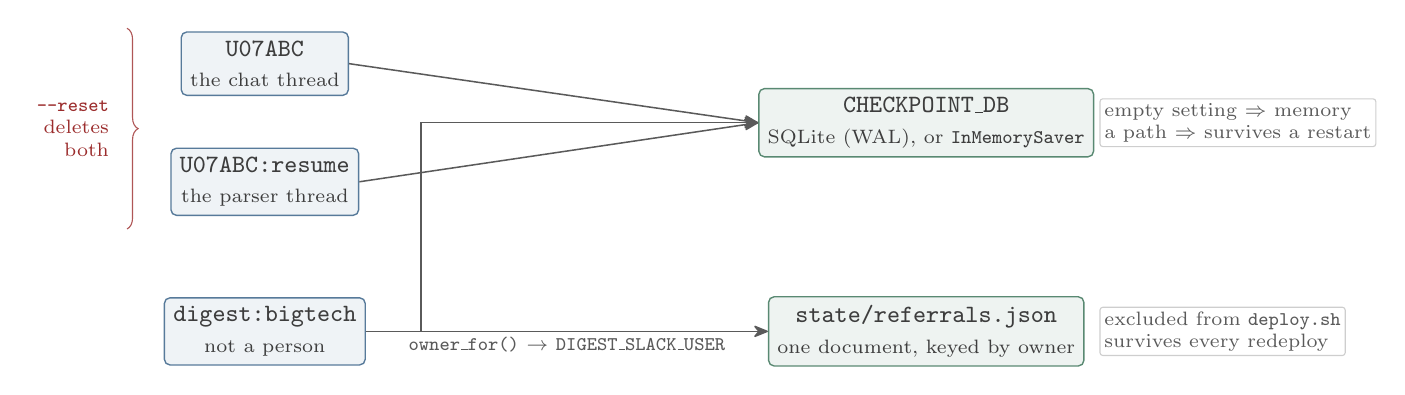
\begin{tikzpicture}[x=1cm,y=1cm]
  \node[core]  (t1)  at (0,0)      {\texttt{U07ABC}\\\scriptsize the chat thread};
  \node[core]  (t2)  at (0,-1.5)   {\texttt{U07ABC:resume}\\\scriptsize the parser thread};
  \node[core]  (t3)  at (0,-3.4)   {\texttt{digest:bigtech}\\\scriptsize not a person};

  \node[state] (db)  at (8.4,-0.75){\texttt{CHECKPOINT\_\allowbreak{}DB}\\\scriptsize SQLite (WAL), or \texttt{InMemorySaver}};
  \node[state] (refs)at (8.4,-3.4) {\texttt{state/referrals.json}\\\scriptsize one document, keyed by owner};

  \draw[flow] (t1.east) -- (db.west);
  \draw[flow] (t2.east) -- (db.west);
  \draw[flow] (t3.east) -- ++(0.7,0) |- (db.west);
  \draw[flow] (t3.east) -- node[lbl,below,pos=0.5]
    {\scriptsize\texttt{owner\_\allowbreak{}for()} $\rightarrow$ \texttt{DIGEST\_\allowbreak{}SLACK\_\allowbreak{}USER}} (refs.west);

  \draw[decorate,decoration={brace,amplitude=4pt,mirror},draw=cWarn!80]
    (-1.75,-2.1) -- (-1.75,0.45)
    node[midway,left=3pt,align=right,font=\scriptsize,text=cWarn]
    {\texttt{-{}-reset}\\deletes\\both};

  \node[lbl, anchor=west, draw=cEdge!25, align=left] at (10.6,-0.75)
    {empty setting $\Rightarrow$ memory\\a path $\Rightarrow$ survives a restart};
  \node[lbl, anchor=west, draw=cEdge!25, align=left] at (10.6,-3.4)
    {excluded from \texttt{deploy.sh}\\survives every redeploy};
\end{tikzpicture}
\end{adjustbox}
\caption{What is stored where, and what a reset destroys. Three thread ids map into one
checkpoint database; the referral list sits outside it on purpose. The digest's thread is not
a Slack user, so \texttt{owner\_\allowbreak{}for()} maps it onto the person the digest is addressed to ---
without that, the morning report would look up a user with no referrals and quietly stop
ranking by them.}
\label{fig:state}
\end{figure}

\begin{table}[!ht]
\centering\tablefont
\caption{The four state stores and their lifetimes.}
\label{tab:state}
\begin{tabularx}{\textwidth}{L{3.2cm} L{3.0cm} L{2.6cm} X}
\toprule
\textbf{Store} & \textbf{Key} & \textbf{Lifetime} & \textbf{Why it is where it is} \\
\midrule
Conversation history & Slack user id & thread, dropped by \texttt{-{}-reset} & It is the
  checkpointer; provider-agnostic messages are what allow a model switch mid-conversation \\
Résumé profile & \texttt{$\langle$user$\rangle$:resume} & same thread lifetime & Caching in
  graph state removes the need for any invalidation logic \\
Referral list & owner (Slack user id) & indefinite & Typed by hand once; must outlive a reset
  and a redeploy \\
Turn metrics & --- & journald retention & One \texttt{key=value} line per turn: greppable,
  no network, always on \\
\bottomrule
\end{tabularx}
\end{table}

Concurrency is handled at three levels and nowhere else. \texttt{slack-bolt} dispatches on a
thread pool; one \texttt{RLock} per user serialises that user's turns while other users run
in parallel. The referral store takes a single process-wide lock, because the per-user locks
order only \emph{one} user's turns and two users editing at once would read-modify-write over
each other. SQLite is opened with \texttt{check\_\allowbreak{}same\_\allowbreak{}thread=False} and a 30-second busy
timeout, in WAL mode so a reader never blocks the writer --- which matters because the digest
process reads the same file while the bot is mid-turn.

One consequence is easy to miss and expensive to discover in production: thread ids are the
bare Slack user id, not namespaced by agent. Two bots pointed at one
\texttt{CHECKPOINT\_\allowbreak{}DB} therefore \emph{share} a thread, and your conversations with them
interleave into one history. Each interactive agent gets its own database path in its own
environment file. The digest was never exposed to this, because its threads are
\texttt{digest:$\langle$key$\rangle$}.

% ==========================================================================
\section{Observability}
% ==========================================================================

Three tiers, with deliberately different costs (Table~\ref{tab:observability}). The design
rule is that the cheapest tier is always on and needs no network, and the expensive tier
cannot break a turn.

\begin{table}[!ht]
\centering\tablefont
\caption{Observability tiers.}
\label{tab:observability}
\begin{tabularx}{\textwidth}{L{2.6cm} L{2.4cm} X L{3.0cm}}
\toprule
\textbf{Tier} & \textbf{Cost} & \textbf{What it answers} & \textbf{Switch} \\
\midrule
Turn metrics & one log line, no network & How long, how many model calls and tool hops, how
  many tokens, which backend answered, and --- when rates are configured --- what it cost &
  always on \\
Langfuse traces & batched export on a background thread & What the turn looked like inside:
  every node, prompt, tool result, latency and token count, grouped by conversation &
  the key pair \emph{is} the switch \\
\texttt{scout doctor} & local reads only & Whether \emph{this checkout} can start, and what
  it will run with less of & a command \\
\texttt{scout stats} & reads the journal & The last $n$ days of turns, aggregated & a command \\
\bottomrule
\end{tabularx}
\end{table}

\paragraph{The key pair is the switch.} There is no separate on/off flag, because a flag can
disagree with the credentials. Half a pair is reported as a warning by \texttt{scout doctor},
because it is the one state that reads as ``on'' in an environment file while tracing
nothing. \texttt{tracing.REQUIRES} is the same tuple the doctor reads, so the report and the
runtime cannot diverge.

\paragraph{Trace names are an API.} \texttt{answer-slack-dm} and \texttt{run-job-digest}
carry no user, agent or model. Langfuse dashboards, saved views and LLM-judge evaluators all
target trace \emph{names}, so anything per-run in a name fragments all three; which agent ran
and on which backend are a tag and a metadata field instead. For the same reason the turn
owns its root span explicitly: trace-level input and output are read off that root, and they
have to be the user's question and the bot's reply --- not LangGraph's message list, which
answers ``what is in the thread'' rather than ``what did it say''. \texttt{Turn.answered()}
is how the reply gets there, including on the stuck path.

\paragraph{Reading the same names the SDK reads.} Langfuse's own client reads
\texttt{LANGFUSE\_\allowbreak{}BASE\_\allowbreak{}URL} ahead of the host passed to its constructor. Reading only
\texttt{LANGFUSE\_\allowbreak{}HOST} therefore had \texttt{scout doctor} confidently reporting the EU
default while traces went to the US endpoint. \texttt{\_\allowbreak{}env\_\allowbreak{}any} now reads the same names in
the same order the SDK does, guarded by \texttt{test\_\allowbreak{}env\_\allowbreak{}any\_\allowbreak{}reads\_\allowbreak{}the\_\allowbreak{}names\_\allowbreak{}in\_\allowbreak{}order}.

% ==========================================================================
\section{Testing strategy}
% ==========================================================================

The suite is 389 tests at 100\,\% statement \emph{and} branch coverage, with
\texttt{fail\_\allowbreak{}under = 100} so the floor is the ceiling, running on Python 3.10 through 3.13
in CI with no credentials and no network access.

That is only possible because there are exactly two stub seams (Table~\ref{tab:testing}).
Chat models are scripted and installed into \texttt{scout.core.models} as if they were real
backends, so the graph reaches them through the same \texttt{build}/\texttt{with\_\allowbreak{}tools}
path it uses for Claude. Every job source's HTTP goes through \texttt{jobs/fetch}, so
stubbing that one module stubs sixteen sources --- which is the practical payoff of making
them all share a fetch layer in the first place.

\begin{table}[!ht]
\centering\tablefont
\caption{What is faked, what is real, and what the suite refuses to do.}
\label{tab:testing}
\begin{tabularx}{\textwidth}{L{3.4cm} L{3.4cm} X}
\toprule
\textbf{Concern} & \textbf{Approach} & \textbf{Why} \\
\midrule
Model providers & \texttt{ScriptedModel} registered as a real backend & The graph, the
  binding and the trimming are all exercised for real; only the network call is not \\
Job-board HTTP & stub \texttt{jobs/fetch.requests} & One seam covers every source, including
  the \texttt{None} contract \\
Slack & the adapter is tested against a fake \texttt{say} & DM filtering, commands and
  message splitting are logic, not I/O \\
Tracing & keys and \emph{both} host names emptied in \texttt{conftest} & The SDK reads
  \texttt{LANGFUSE\_\allowbreak{}BASE\_\allowbreak{}URL} itself; one test was otherwise posting to Langfuse Cloud \\
LangSmith & \texttt{LANGSMITH\_\allowbreak{}TRACING=false} pinned & Not Scout's setting at all ---
  \texttt{langsmith} ships with \texttt{langchain-core} and reads it, so a stale
  \texttt{.env} could export traces from a test run \\
Developer environment & settings pointed at \texttt{tmp\_\allowbreak{}path} & A test that reads the
  author's own \texttt{.env} or \texttt{data/} passes locally and fails in CI \\
Packaging & \texttt{test\_\allowbreak{}packaging.py} & \texttt{requirements*.txt} are generated from
  \texttt{pyproject.toml}; the Dockerfile installs from the flat list, so drift is a
  deployment bug \\
Documentation & \texttt{test\_\allowbreak{}docs.py} & Every relative link and heading anchor in every
  Markdown file must resolve \\
\bottomrule
\end{tabularx}
\end{table}

Two habits do most of the work. First, the test names are sentences about behaviour
(\texttt{test\_\allowbreak{}every\_\allowbreak{}board\_\allowbreak{}being\_\allowbreak{}down\_\allowbreak{}is\_\allowbreak{}not\_\allowbreak{}reported\_\allowbreak{}as\_\allowbreak{}nothing\_\allowbreak{}open}), so a failure
report names the property that broke rather than the function that threw. Second, the
invariants that are easy to break silently have a test each, named after the invariant ---
which is why the decision log above can cite one for nearly every row.

% ==========================================================================
\section{Deployment and operations}
\label{sec:deploy}
% ==========================================================================

The whole platform is six systemd units on one free-tier instance
(Figure~\ref{fig:deploy}), configured by a four-layer precedence chain
(Table~\ref{tab:config}).

\begin{figure}[!ht]
\centering
\begin{adjustbox}{max width=\textwidth}
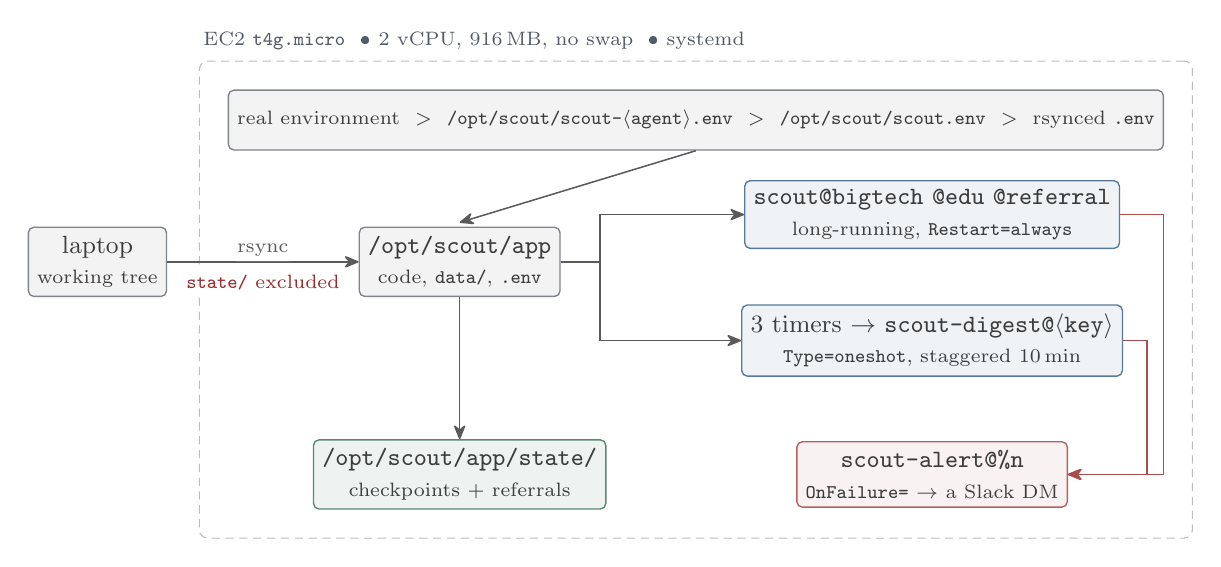
\begin{tikzpicture}[x=1cm,y=1cm]
  \node[infra] (laptop) at (0,-1.6) {laptop\\\scriptsize working tree};
  \node[infra] (app)    at (4.6,-1.6){\texttt{/opt/scout/app}\\\scriptsize code, \texttt{data/}, \texttt{.env}};
  \node[infra, minimum width=96mm, font=\scriptsize] (envs) at (7.6,0.2)
    {real environment \ $>$ \ \texttt{/opt/scout/scout-$\langle$agent$\rangle$.env} \ $>$ \
     \texttt{/opt/scout/scout.env} \ $>$ \ rsynced \texttt{.env}};

  \node[core]  (bots)   at (10.6,-1.0) {\texttt{scout@bigtech} \texttt{@edu} \texttt{@referral}\\\scriptsize long-running, \texttt{Restart=always}};
  \node[core]  (timers) at (10.6,-2.6) {3 timers $\rightarrow$ \texttt{scout-digest@$\langle$key$\rangle$}\\\scriptsize \texttt{Type=oneshot}, staggered 10\,min};
  \node[warn]  (alert)  at (10.6,-4.3) {\texttt{scout-alert@\%n}\\\scriptsize \texttt{OnFailure=} $\rightarrow$ a Slack DM};
  \node[state] (state)  at (4.6,-4.3)  {\texttt{/opt/scout/app/state/}\\\scriptsize checkpoints $+$ referrals};

  \draw[flow] (laptop) -- node[lbl,above]{\scriptsize rsync}
              node[faillbl,below=1mm]{\scriptsize\texttt{state/} excluded} (app);
  \draw[flow] (app.east) -- ++(0.5,0) |- (bots.west);
  \draw[flow] (app.east) -- ++(0.5,0) |- (timers.west);
  \draw[flow] (app) -- (state);
  \draw[flow] (envs.south) -- (4.6,-1.1);
  \draw[fail] (bots.east) -- ++(0.55,0) |- (alert.east);
  \draw[fail] (timers.east) -- ++(0.3,0) |- (alert.east);

  \begin{scope}[on background layer]
    \node[grp, fit=(app)(bots)(timers)(alert)(state)(envs)] (box) {};
  \end{scope}
  \node[grplbl, anchor=south west] at ([yshift=0.8mm]box.north west)
    {EC2 \texttt{t4g.micro} \ \textbullet\ 2 vCPU, 916\,MB, no swap \ \textbullet\ systemd};
\end{tikzpicture}
\end{adjustbox}
\caption{Deployment topology. Both service files are systemd \emph{templates}: a second agent
is \texttt{systemctl enable scout@edu}, not a second unit file. The precedence chain at the
top is what lets host-local secrets outrank the rsynced \texttt{.env} without either file
knowing about the other.}
\label{fig:deploy}
\end{figure}

\begin{table}[!ht]
\centering\tablefont
\caption{Configuration surface. The rule is that anything which cannot be shared between
agents goes in the per-agent file, and everything else stays in one place.}
\label{tab:config}
\begin{tabularx}{\textwidth}{L{3.6cm} L{3.4cm} X}
\toprule
\textbf{Layer} & \textbf{Holds} & \textbf{Precedence and reason} \\
\midrule
Process environment & \texttt{AGENT}, anything systemd sets & Highest.
  \texttt{load\_\allowbreak{}dotenv} never overrides an existing key, so the deployed
  \texttt{EnvironmentFile} stays authoritative over a rsynced file \\
\texttt{.env.$\langle$agent$\rangle$} & Slack token pair, \texttt{CHECKPOINT\_\allowbreak{}DB} & Each
  agent is its own Slack app; each interactive agent needs its own database path \\
\texttt{.env} & API keys, limits, model names, Langfuse & Shared by every agent; never
  copied per agent \\
\texttt{AgentSpec} & prompt, tools, default backend, behaviour flags & Configuration that is
  code, because it is reviewed like code \\
\bottomrule
\end{tabularx}
\end{table}

\texttt{deploy.sh} ships the working tree with rsync rather than doing a \texttt{git pull} on
the box, for a specific reason: \texttt{.env} and \texttt{data/} are git-ignored but are
exactly what the host needs, so one copy covers code, résumé and secrets. The cost is that
the box has no git history to identify itself with, so the script records the branch, the
short revision and whether the tree was dirty into \texttt{/opt/scout/DEPLOYED}. Untracked
files count as dirty, because rsync sends them and they then run on the box without appearing
in any commit.

Two operational details are worth stating because they are the kind an interviewer probes.
Socket Mode holds a websocket, and container platforms and systemd stop a process with
\texttt{SIGTERM}, which by default kills Python outright --- the socket is never closed and
the shutdown path never runs. Scout installs a handler that raises
\texttt{KeyboardInterrupt}, so \texttt{SIGTERM} unwinds through exactly the same path as
Ctrl-C. And alerting goes to Slack rather than CloudWatch because the box has no IAM role;
an alert that requires opening a console is an alert nobody reads. \texttt{Restart=always}
means a single restart is normal and silent --- systemd only reports failure once a unit
exceeds its restart burst, which is the signal actually worth a notification. A bot that is
running but has silently lost its websocket still looks healthy to systemd; the daily digest
is the backstop for that, because if it stops arriving, something is wrong.

% ==========================================================================
\section{Limits, and what the next constraint would be}
% ==========================================================================

Table~\ref{tab:limits} is the list of things this design does not do, in the order in which
they would actually start to hurt.

\begin{table}[!ht]
\centering\tablefont
\caption{Known limits, ordered by how soon each would actually bite.}
\label{tab:limits}
\begin{tabularx}{\textwidth}{L{3.5cm} X L{4.2cm}}
\toprule
\textbf{Limit} & \textbf{Why it exists} & \textbf{What would remove it} \\
\midrule
Single box, no redundancy & One \texttt{t4g.micro}; a reboot is downtime & Two instances
  behind nothing at all --- Socket Mode means no load balancer, so it is an
  active/standby problem, not a routing one \\
Memory ceiling & 916\,MB, no swap, three resident processes & Staggering already covers the
  digests; a fourth interactive agent needs a bigger instance \\
Digest dedupe is prose-based & Agents return text, so the structured \texttt{JobPosting}
  objects are gone by reply time; the only dedupe is the model reading its own thread &
  Have the digest call the searchers directly and render in code, keeping the model for
  ranking only \\
No rate limiting toward boards & A referral sweep issues up to four concurrent requests and
  runs daily; nobody has complained & A token bucket in \texttt{fetch}, which is the single
  choke point every source already passes through \\
Company coverage is hand-maintained & \texttt{directory.py} is a table by design & Nothing
  --- this is the cost of the completeness guarantee, and it is the right trade \\
Single user in practice & Per-user locks and per-user threads exist, but there is one Slack
  workspace and one résumé directory & Résumé storage per user, and a real secret store
  rather than environment files \\
\bottomrule
\end{tabularx}
\end{table}

The honest summary is that the architecture is sized for its actual problem. The seams that
exist --- agent, tool, source, provider --- are the four axes along which this system has in
fact changed, repeatedly; there is no abstraction layer waiting for a second user, a second
workspace, or a database that is not SQLite, because none of those has been needed and each
would have cost clarity now for flexibility later.

\appendix
% ==========================================================================
\section{Interview cheat sheet}
% ==========================================================================

\begin{enumerate}[leftmargin=1.4em,itemsep=5pt]
  \item \textbf{``Walk me through the architecture in two minutes.''} Slack DM adapter
    $\rightarrow$ \texttt{ConversationalAgent} $\rightarrow$ a LangGraph model/tool loop
    that every agent compiles to $\rightarrow$ tools, of which sixteen are job sources over a
    shared fetch/render/relevance layer. An agent is a declarative spec, history is a
    checkpointer thread per user, and everything else --- the digest, the tracing, the
    fallback --- hangs off those three facts.

  \item \textbf{``Why LangGraph and not just a loop?''} I had the loop first. LangGraph
    bought checkpointing, subgraphs and a tool node, and it made tool traffic part of history
    so the model remembers what it looked up. The cost is that tool messages consume the
    context window, which is a trade I would make again.

  \item \textbf{``How does a user switch models mid-conversation?''} History is stored as
    provider-agnostic LangChain message objects, not as any vendor's wire format, so the
    thread replays into whichever integration is chosen. The backend rides in the graph
    config per turn, so one compiled graph serves every user on every model.

  \item \textbf{``What happens when a job board is down?''} It returns \texttt{None}, never
    an empty list, and the reply names it as unchecked. That distinction is the whole
    reason the Referral Window's answer can be trusted --- ``nothing open'' where the truth
    is ``I could not look'' is what sends someone away from a company they should have asked.

  \item \textbf{``Why not let the model figure out which board a company is on?''} It gets it
    right most of the time, and most of the time is exactly what a completeness claim cannot
    be. Routing in code is also what makes it possible to \emph{name} the companies that have
    no board, instead of silently dropping them.

  \item \textbf{``How do you stop it hallucinating a posting date?''} Two sources publish no
    date at all and several publish only relative wording. Those go into a separate
    \texttt{posted\_\allowbreak{}label} field that is never coerced into a timestamp, undated postings sort
    last, and the digest prompt says to repeat the tool's wording verbatim or write ``no date
    given''.

  \item \textbf{``What breaks if a turn runs out of tool calls?''} Without the repair, the
    user's \emph{next} message --- because the thread would contain tool calls with no
    results, which providers reject. \texttt{\_\allowbreak{}give\_\allowbreak{}up()} writes a synthetic result for each
    abandoned call before recording the apology.

  \item \textbf{``Where does the retry live, and why does that matter?''} Inside the model
    node. A node that raises commits nothing, so the retry starts clean while keeping tool
    results the turn already fetched. Retrying around the turn would either discard that work
    or hammer a dozen careers boards twice.

  \item \textbf{``How do you keep an agent from doing something the user did not ask for?''}
    Capability, not instruction. Job agents import a read-only referral module, so the write
    tools are not in their schema at all. The one agent that may write has no tool to search
    off-list with. Both are pinned by tests named after the invariant.

  \item \textbf{``How is it tested without network access?''} Two stub seams: chat models are
    scripted and registered as real backends, and every source's HTTP goes through one fetch
    module. 389 tests, 100\,\% statement and branch coverage, Python 3.10--3.13, no
    credentials in CI.

  \item \textbf{``What does observability cost you per turn?''} The always-on tier costs one
    log line and no network. Tracing is opt-in, built lazily on the first traced turn, and
    exported in batches on a background thread --- and if it cannot start, it logs once and
    the process runs untraced. No branch in the graph knows either way.

  \item \textbf{``What would you change?''} Render the digest in code from the structured
    postings rather than asking the model to reformat them --- that would give real dedupe
    instead of relying on the model reading its own thread --- and put a token bucket in the
    fetch layer before coverage grows further.
\end{enumerate}

% ==========================================================================
\section{The sixty-second version}
% ==========================================================================

\noindent
Scout is a multi-agent job-search assistant that lives in Slack DMs. Each agent is a system
prompt plus a set of tools, declared in one file and compiled onto a shared LangGraph
model/tool loop; adding an agent never touches the graph. Job agents run behind a résumé
parser whose output is cached in checkpointed graph state, so the résumé is parsed once per
thread and every search is tailored without the user restating anything. Sixteen source
modules cover twenty-nine companies over one shared HTTP, rendering and relevance layer, and
each exposes its search twice --- as a tool for the model, and as a plain function so a third
agent can sweep every company where the user has a referral and say exactly which boards it
could not reach. The whole thing runs as six systemd units on a free-tier EC2 instance, with
one log line per turn always on, optional Langfuse tracing that cannot break a turn, and a
test suite that runs at 100\,\% branch coverage with no network and no credentials.

\end{document}
